\section{Daten}
\subsection{Stichproben und Merkmale}
\begin{wrapfigure}[12]{r}{0.2\textwidth}
    \centering
    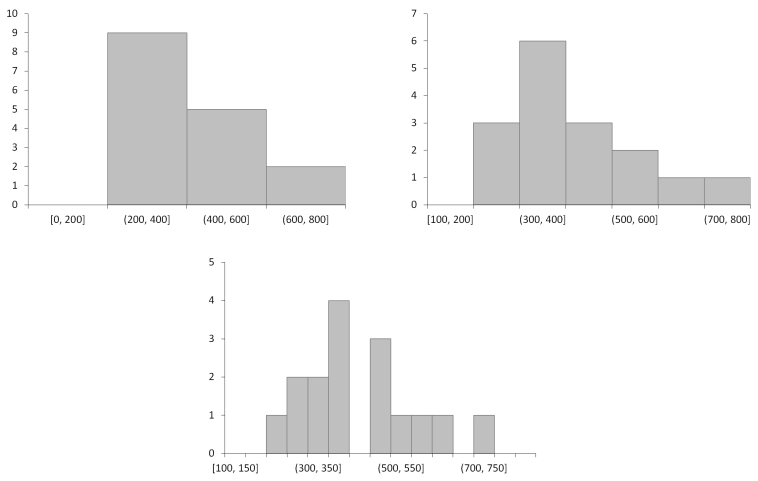
\includegraphics[width=0.2\textwidth]{images/2.2_histogramme.png}
    \caption{Verteilungen mit unterschiedlichen \emph{Partitionen}}
    \label{fig:histogramme-binning}
    
\end{wrapfigure}
Elemente einer Stichprobe b(z. B. Umfrageteilnehmer) werden als statische \hlc{Einheiten} oder \hlc{Merkmalsträger} bezeichnet.
Die von ihnen erhobenen Daten bezeichnet man als \hlc{Merkmale} oder \hlc{Variablen} (z.b. Geschlecht, Alter, Monatliches Einkommen...). 
Man unterscheidet hierbei zwischen \hlc{Zielgrößen} die von anderen Variablen abhängen, \hlc{Einflußgrößen} bzw. \hlc{Faktoren}, die beobachtet werden können und \hlc{Störgrößen, die als latente Größen nicht beobachtbar sind}.
\subsection{Merkmalstypen}
Ein Merkmal heißt \hlc{diskret} wenn es nur \emph{endlich} oder \emph{abzählbar} unendlich viele mögliche Ausprägungen besitzt (z. B. Anzahl Personen in einer Wohneinheit). Merkmale, die \emph{überabzählbar} viel Werte annehmen können werden als \hlc{stetig}  bezeichnet (z. B. ein Messwert wie Temperatur). Aufgrund von Messungenauigkeiten und/oder Rundungen können \emph{stetige} Werte \emph{diskret} werden. Man spricht von \hlc{quasi-stetigen} Werten. 
\\\\
Merkmale lassen sich auch bzgl. der \hlc{Skalen} unterscheiden, auf denen ihre Ausprägung gemessen werden. \hlc{Nominalskala}: Die Ausprägungen entsprechen Namen oder Kategorien, beispielsweise das Geschlecht oder der Typ der Unterkunft. \hlc{Ordinalskala}: Ausprägungen besitzen eine natürliche \emph{Ordnung}, \emph{ohne} dass
die Abstände interpretierbar sind. Dies gilt beispielsweise bei Wohnungen für die Entfernung zum Campus oder Notenstufen (-> Rechnungen ergeben keinen Sinn). 
\hlc{Kardinalskala}: Ausprägungen sind Zahlen, sodass auch die Abstände im Kontext von Differenzen oder Quotientenbildung interpretierbar sind (z. B. Miete, Quadratmeter -> Miete pro Quadratmeter).
Man kann durch Datentransformation von einer feineren auf eine Skala mit geringeren Informationsgehalt wechseln (Bsp Gruppierung von Entfernungen zum Campus: 3km, 5km, 10km etc.).
\\\\
Ein Merkmal heißt \hlc{qualitativ} oder \hlc{kategorial}, wenn es nur endlich viele Ausprägung Besitz und diese höchstens \emph{ordinal} skaliert sind.
Anderenfalls ist ein Merkmal \hlc{quantitativ}.


\section{Univariate Datenanalyse}
Univariate Daten $\rightarrow$ Merkmale werden als unabhängig angenommen und für einzeln ausgewertet. Häufigkeiten. Stichprobe besteht aus n statistischen Einheiten und $x_1, ..., x_n$ bezeichnet die \emph{beobachteten} Ausprägungen eines Merkmals $X$. $a_1, ..., a_k$ bezeichnet die Menge der \emph{unterschiedlichen} Ausprägungen, die in der Stichprobe beobachtet wurden.
\subsection{Häufigkeiten}
Die \hlc{absolute Häufigkeit} $h(a_j) = h_j$ bezeichnet nun die Anzahl an Beobachtungen des jeweiligen Merkmals $a_j$. \hlcm{$h(a_i) = h_j := \sum^{n}_{i=1}\mathds{1}(x_i)$} ($\mathds{1}(x_i)$ $\rightarrow$ Indikatorfunktion $\rightarrow$ wenn $a_j == x_i 1$ sonst $0$). \hlc{Relative Häufigkeit} ist die absolute Häufigkeit bezogen auf die Größe der Stichprobe \hlcm{$f(a_j) = f_j := \frac{h_j}{n}$} 
\begin{wrapfigure}{l}{0.2\textwidth}
    \centering
    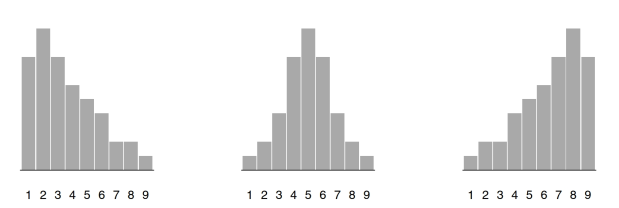
\includegraphics[width=0.2\textwidth]{images/2.3_histogramme_schiefheit.png}
    \caption{linkssteile/rechtsschiefe (links), symmetrische (Mitte) und rechtssteile/linksschiefe
    (rechts) Verteilungen}
    \vspace{-12mm}
    \label{fig:schiefheit}
\end{wrapfigure}
Hat ein Histogramm wie in \cref{fig:schiefheit} einen klaren Höhepunkt spricht man von einer \hlc{unimodalen} Verteilung, bei zwei von einer \hlc{bimodalen}- und bei mehr als zwei Höhepunkten von einer \hlc{multimodalen} Verteilung. Auch wird normalerweise die \hlc{Steilheit} benannt (\cref{fig:schiefheit}).
Die \hlc{Kummulierte Häufigkeitsverteilung} \hlcm{$H(x):=\sum^{n}_{i=1}\mathds{1}_{\{x_i \leq x\}} = \underset{j:a_j\leq x}{\sum}h(a_j)$}gibt an, wie viele der Beobachtungen $x_1, ..., x_n$ kleiner oder gleich x sind und analog ergibt sich die \hlc{empirische Verteilungsfunktion} \hlcm{$F(x) := \frac{H(x)}{n} = \frac{1}{n}\sum^{n}_{i=1}\mathds{1}_{\{x_i \leq x\}} = \underset{j:a_j\leq x}{\sum}f(a_j)$} durch die Normierung von $H(x)$ auf die Grundgesamtheit der Stichprobe. Kumulierte Häufigkeitsverteilungen sind monoton wachsende und rechtsseitig stetige Treppenfunktionen, mit Treppenstufen bei jeder Ausprägung $a_j$ und in der Höhe $h_j$ bzw. $f_j$. Bsp. \glqq Wie häufig leben \emph{höchstens} 3 Personen zusammen?\grqq $\rightarrow$ $F(3) = 3/4$  \glqq Wie häufig leben \emph{mindestens} 2 Personen zusammen?\grqq $\rightarrow$ $1 - F(1) = \frac{13}{16}$ (Werte für F aus Verteilung/Tabelle berechenbar oder aus Diagram ablesbar).
\\\\ 
\subsection{Lagemaße}
Das \hlc{arithmetisches Mittel} $\bar{x} := \sum^n_{i=1}$ ist zwar anschaulich leicht verständlich, jedoch sehr anfällig gegenüber Ausreißern. Ein stabileres Lagemaß ist der \hlc{Median}. Er ist dadurch charakterisiert, dass (mindestens) die Hälfte der Daten größer oder gleich und (mindestens) die Hälfte der Daten kleiner oder gleich seinem Wert ist. \hlcm{$x_{med} = \begin{cases} x_{(\frac{n+1}{2})} & \text{,falls }n \text{ ungerade} \\
\frac{1}{2}(x_{(\frac{n}{2})} + x_{(\frac{n+1}{2})}) & \text{,falls }n \text{ gerade}
\end{cases}$.} Der \hlc{Modus} \hlcm{$x_{mod} := \underset{a_j}{\text{arg }\text{max }}h(a_j) =\underset{a_j}{\text{arg }\text{max }}f(a_j)$} entspricht dem Element, dass am häufigsten in einer Verteilung auftritt. Für die drei Lagemaße gilt: \emph{Symmetrische Verteilung}: $\bar{x}=x_{med}=x_{mod}$. \emph{Linkssteile/rechtsschiefe Verteilung}: $\bar{x} > x_{med} > x_{mod}$. \emph{Rechtssteile/linksschiefe Verteilung}: $\bar{x}<x_{med}<x_{mod}$. 
Für \hlc{Wachstumsprozesse} ist das \hlc{gemetrische Mittel} ebenfalls von Interesse. Seien $x_1, ..., x_n$ die \emph{Wachstumsfaktoren} über $n$ Perioden, dann ergibt sich aus einem \emph{Ausgangswert}\linebreak$B_0$: $B_n = B_0 \Pi_{i=1}^nx_i$. Das \emph{geometrische Mittel} ist nun der \emph{konstante} Wachstumsfaktor,  für den gilt: $B_n = B_0\,\bar{x}_{geom}^n$. Aus gleichstellen der beiden Gleichungen folgt: \hlcm{$\bar{x}_{geom} = (\Pi_{i=1}^n x_i)^{1/n}$}. Ausgehen von Wachstumsraten $r_i = x_i - 1$ liefert das \emph{geometrische Mittel} die \hlc{durchscnittliche Wachstumsrate} $\bar{r}_{geom} = (\Pi_{i=1}^n(1+r_i))^{1/n}$. 
Je nach Fragestellung kann auch das \hlc{harmonische Mittel} ein geeigneter Mittelwert sein \hlcm{$\bar{x}_{harm}=\frac{1}{\frac{1}{n}\sum_{i=1}^n\frac{1}{x_i}}$}. \hlc{Ein Bsp. wären $n$ verschiedene Bauteile die eine Produktionslinie der Länge $l$ mit den Geschwindigkeiten $x_1, ..., x_n$} nacheinander durchlaufen: $\bar{x}_{harm} = \frac{l + ... + l}{\frac{l}{x_1} + ... + \frac{l}{x_n}}$.
\begin{wrapfigure}{r}{0.3\textwidth}
    \centering
    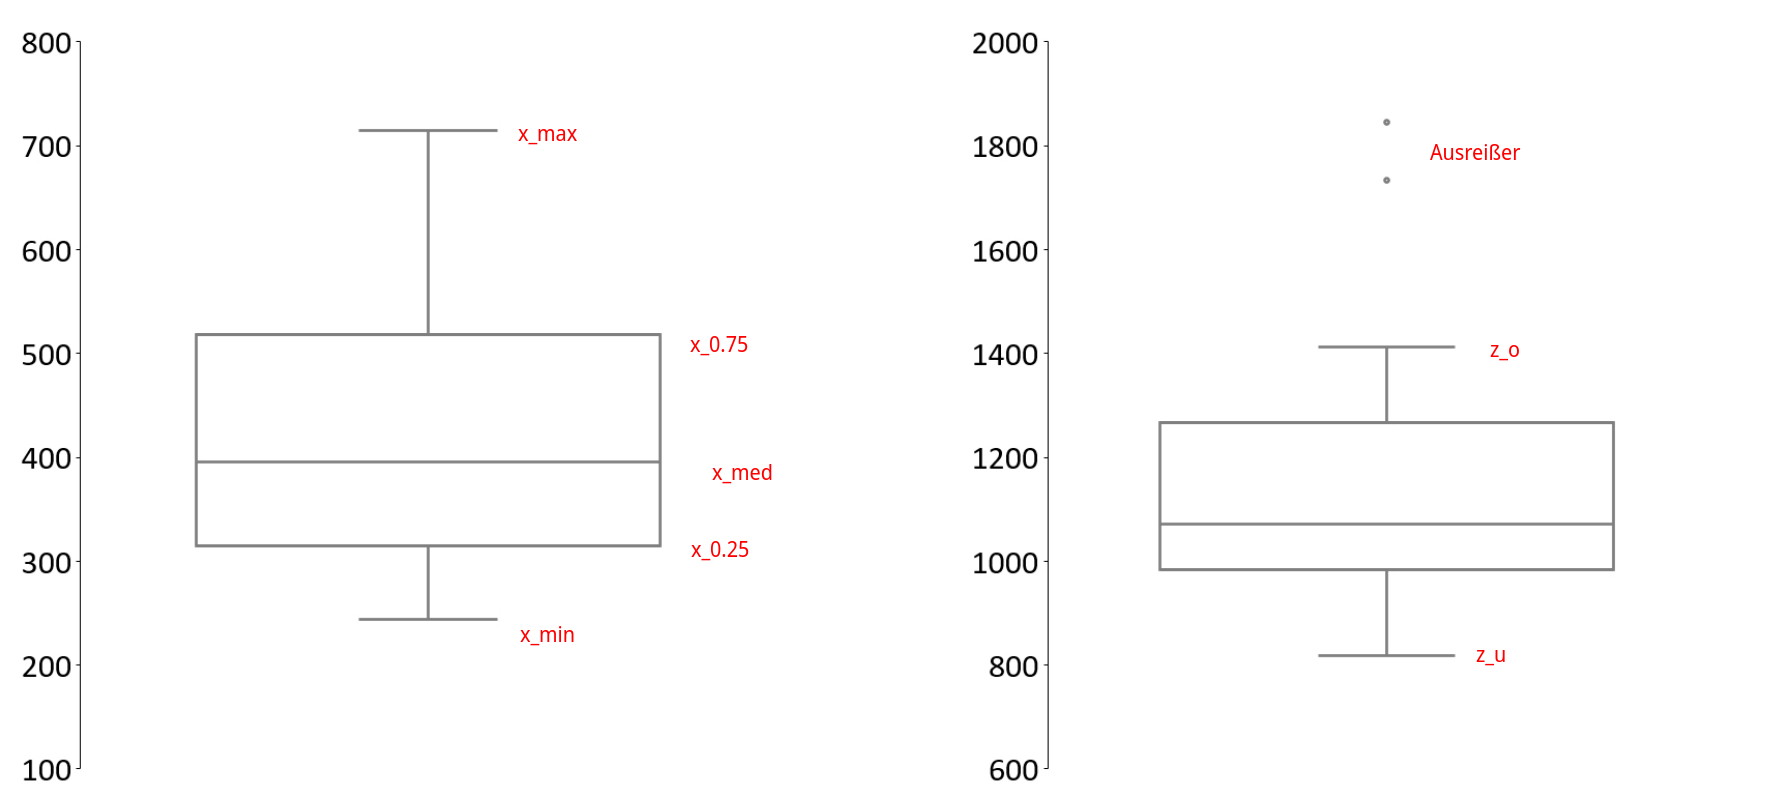
\includegraphics[width=0.3\textwidth]{images/2.5_boxplot.png}
    \caption{Box-Whisker Plot}
    \vspace{-10mm}
    \label{fig:boxplot}
\end{wrapfigure}
Bei der Auswertung einer Verteilung ist neben dem Zentrum auch die Frage relevant, in wie weit einzelne Beobachtungen vom Zentrum abweichen. \hlc{Quantile} bieten insbesondere die Möglichkeit, die Lage von besonders großen oder kleinen Beobachtungen anzugeben. Das \hlc{p-Quantil} mit $p \in [0, 1]$ für \emph{aufsteigend geordneten} Beobachtungen $x_{(1)}, ..., x_{(n)}$ eines Merkmals $X$ wird mit \hlcm{$x_p = \begin{cases} x_{(\floor{n\cdot p} + 1)} & \text{,falls }n \text{ \emph{nicht} ganzzahlig} \\
    \frac{1}{2}(x_{(n\cdot p)} + x_{(n\cdot p + 1)}) & \text{,falls }n\cdot p \text{ ganzzahlig}
    \end{cases}$} bestimmt.
    
\subsection{Streuungsmaße}
Die \emph{Breite \emph{bzw.} Streuung einer Verteilung} ist die sog. Spannweite oder \emph{span}. Sie ergibt sich durch \hlcm{$span = \text{max }\{x_1, ...,\,x_n\} - \text{min }\{x_1, ...,\,x_n\} = x_{(n)} - x_{(1)}$}. Da span jedoch sehr anfällig gegenüber Ausreißern ist verwendet man idr den \hlc{Interquantilsabstand \emph{IQR}} er ergibt sich aus \hlcm{$d_Q = x_{0.72} - x_{0.25}$}. Durch die Definition der Quantile liegt innerhalb seiner Grenzen, die \glqq mittlere Hälfte\grqq einer Beobachtung. \hlc{Ausreißer} sind Punkte, die sich nicht in \hlcm{$[z_u, z_o]$}, mit $z_u = x_{0.25} - 1.5dQ$ und $z_o = x_{0.75} + 1.5dQ$ befinden. Die \hlc{Zusammenfassung einer Verteilung} ist durch $x_{(1)}\text{, }x_{0.25}\text{, }x_{med}\text{, }x_{0.75}\text{, }x_{n}$ definiert. In \cref{fig:boxplot} ist die Zusammenfassung als Boxplot zu sehen.\linebreak\\
Seien $x_1, ..., x_n$ die Beobachtungen eines Merkmals $X$. Dann ist die \hlc{Stichprobenvarianz} \hlcm{$s^2 = s_X^2 := \frac{1}{n-1} \sum_{i=1}^n(x_i - \bar{x})^2 = \frac{1}{n-1} \sum_{j=1}^k(a_j - \bar{x})^2 \cdot h_j $}. Die \hlc{Stichprobenstandardabweichung} ergibt sich durch \hlcm{$s = \sqrt{s^2}$}. Sie lässt sich, wie der name schon vermuten lässt als \glqq standardmäßige Abweichungen\grqq\, der einzelnen Beobachtungen vom arithmetischen Mittel interpretieren. der Grund für die Division durch \emph{$n-1$} und nicht durch \emph{$n$} ist, dass die Abweichung nicht bzgl. dem tatsächlichen Mittelwert der zugrundeliegenden Population sondern dem arithmetischen Mittelwert der Stichprobe bestimmt wird. Da dieser Wert \glqq optimal\grqq\, zur Stichprobe passt, werden die Abweichung zum tatsächlichen Mittelwert systematisch unterschätzt.Mit dem \emph{Verschiebungssatz} gilt außerdem \hlcm{$s^2 = \frac{1}{n-1}\sum_{i=1}^nx_i^2 - \frac{n}{n-1}\bar{x}^2$}. Für den \emph{Vergleich von Streuungen} bzw. die Berechnung der \hlc{relativen Streueung} wird der \hlc{Variationskoeffizient} benutzt: \hlcm{$v = \frac{s}{\bar{x}}$}
\section{Multivariate Datenanalyse}
\begin{wrapfigure}{l}{0.2\textwidth}
    \vspace{-5mm}
    \centering
    \includegraphics[width=0.2\textwidth]{images/gemeinsame_häufigkeit_rel_bsp.png}
    \caption{Kontingenztafel für relative Häufigkeiten für Merkmal Geschlecht und Wohnungstyp}
    \label{fig:kontingenztafeln}
    \vspace{-9mm}
\end{wrapfigure}
Oft kommt es vor, dass Merkmale nicht unabhängig voneinander sind sondern zusammenhänge Zwischen ihnen bestehen.

\subsection{Zweidimensionale Merkmale}
\subsubsection{Diskrete Merkmale}
\textbf{Gemeinsame Häufigkeiten:} Die gemeinsame Verteilung zweier diskreterer Merkmale kann mit Hilfe einer \hlc{Kontingenztafel} vgl. \cref{fig:kontingenztafeln} aufbereitet und veranschaulicht werden. Dabei werden die Ausprägungen $a_1, ..., a_k$ und $b_1, ..., b_m$ der Merkmale $X$ und $Y$ wie in \cref{fig:kontingenztafeln} aufgetragen. Die Einträge im inneren der Tafel ergeben sich durch $h_{ij} = h(a_i, b_j)$ (D.h. die Anzahl Beobachtungen an denen \emph{beide} Ausprägungen zu sehen sind) bzw. durch $f_{ij} = \frac{h_{ij}}{n}$. In der letzten Spalte stehen die \hlc{Randhäufigkeiten} des Merkmals $X$. Sie ergeben sich aus der Summe der Einträge der jeweiligen Zeile. Anschaulich Handelt es sich dabei um die Häufigkeit der Ausprägung $a_1, ..., a_k$, ohne Berücksichtigung des Merkmals $Y$ erhält. In Summe ergeben sie $n$ bzw. $1$. Gleiches gilt für die letzte Zeile.\linebreak\\
\textbf{Bedingte Häufigkeiten:} Ausgehend von gemeinsamen Häufigkeiten zweier Merkmale möchte man gelegentlich auch die Verteilung eines Merkmals angeben unter der Bedingung, dass das andere Merkmal auf eine konkrete Ausprägung fixiert ist. In dem Fall spricht man von einer \emph{bedingten Häufigkeitsverteilung}. \hlc{Die bedingte Häufigkeitsverteilung von Y unter der Bedingung $X = a_i$ , kurz $Y |X = a_i$} , ist gegeben durch die relativen Häufigkeiten \hlcm{$f_{Y|X=a_i}(b_1)=\frac{h_{i1}}{h_i.}, ..., f_{Y|X=a_i}(b_m)=\frac{h_{im}}{h_i.}$}. Analog ist die \hlc{bedingte Häufigkeitsverteilung von X unter der Bedingung $Y = b_j$ , kurz $X|Y = b_j$} gegeben als \hlcm{$f_{X|Y=b_j}(a_1)=\frac{h_{1j}}{h_{.j}}, ..., f_{X|Y=b_j}(a_k)=\frac{h_{kj}}{h_{.j}}$}
\subsubsection{Stetige Merkmale}
\begin{wrapfigure}{r}{0.3\textwidth}
    \vspace{-8mm}
    \centering
    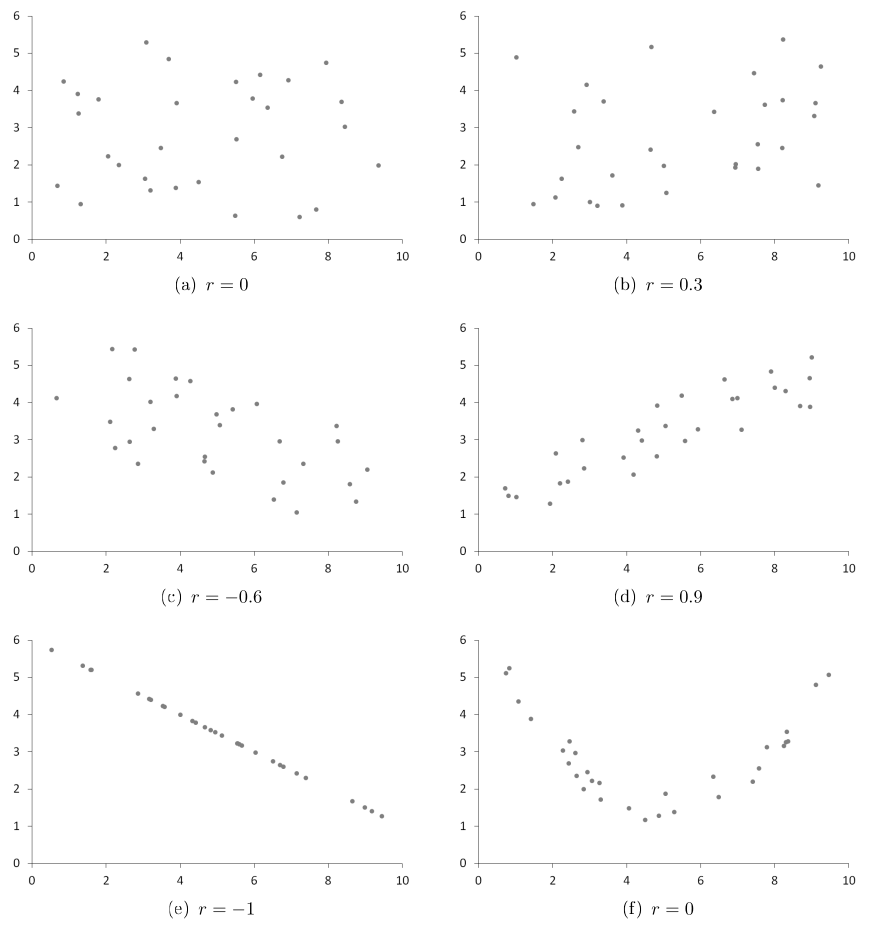
\includegraphics[width=0.3\textwidth]{images/3.4_streudiagramme_mit_unterschiedlicher_kor.png}
    \caption{streudiagramme für STichproben mit verschiedenen Korrelationen}
    \vspace{-12mm}
    \label{fig:streudiagramme}
\end{wrapfigure}
Die einfachste Möglichkeit, die gemeinsamen Beobachtungen stetiger Merkmale darzustellen, ist das Streudiagramm, bei dem alle Beobachtungen als Punkte in der $(x, y)$ -Ebene aufgetragen werden. Dabei genügt es, dass ein Merkmal stetig und das andere zumindest ordinalskaliert ist, um übereinander liegende Punkte (weitestgehend) auszuschließen. Diese Diagramme vermitteln einen schnellen Eindruck, ob es möglicherweise einen Zusammenhang zwischen den beiden Merkmalen gibt und, wenn ja, ob dieser positiv (steigende Gerade) oder negativ (fallende Gerade) ist.

\subsection{Quantifizierung von Zusammenhängen}
Für eine zweidimensionale Stichprobe $(x_1, y_1), ..., (x_n, x_n)$ der Merkmale $X$ und $Y$ ist die \emph{Stichprobenvarianz} \hlcm{$s_{XY}^2 := \frac{1}{n-1}\sum_{i=1}^n(x_i - \bar{x}) (y_i - \bar{y})$}. Eine \hlc{positive Stichprobenvarianz} deutet auf einen positiven (d.h. linearen bzw. proportionalen) Zusammenhang Zusammenhang zwischen den Merkmalen hin und man sagt, dass die Merkmale \emph{positiv korreliert} sind. Analog deutet eine \hlc{negative Stichprobenvarianz} auf einen negativen (bzw. indirekt proportionalen) Zusammenhang hin, man spricht von \emph{negativer Korrelation}. Bei einer \hlc{Stichprobenvarianz nahe null} ist kein klarer (linearer) Zusammenhang erkennbar und die Merkmales sind (näherungsweise) \emph{unkorreliert}.\\\\

Zwar kann man am Vorzeichen der Stichprobenvarianz eine Tendenz erkennen allerdings bietet die Stichprobenvarianz keine Möglichkeit die stärke der Korrelation zu messen bzw. zu vergleichen. Um das zu erreichen wird die Stichprobenvarianz auf das Produkt der Stichprobenstandardabweichungen der einzelnen Merkmale normiert. Der so entstehende \hlc{Bravais-Person-Korrelationskoeffizient} ist definiert durch \hlcm{$r = r_{XY} := \frac{s_{XY}^2}{s_X \cdot s_Y}$}. Der Bravais-Pearson-Korrelationskoeffizient hat folgende Eigenschaften, die in \cref{fig:streudiagramme} veranschaulicht werden:
\begin{itemize}[leftmargin=*]
    \itemsep0em 
    \item Aufgrund der Normierung gilt $-1 \le r \le 1$ Ein Wert $|r|~=1$ weißt auf eine starke Korrelation hin. Die Grenzen sind allerdings fließend. Häufig spricht man bei $|r| < 0.5$ von einer schwachen  Korrelation, bei $0.5 < r < 0.8$ von einer mittleren Korrelation und bei $|r| \ge 0.8$ von einer starken Korrelation.
    \item Es gilt $r_{XY} = r_{YX}$, da der Korrelationskoeffizienten nur die Stärke des Zusammenhangs und nicht dessen Richtung misst.
    \item Der Korrelationskoeffizient misst, genau wie die Stichprobenkovarianz, die lineare Abhängigkeit zwischen den Merkmalen X und Y . Diese Linearität lässt sich wie folgt ausdrücken: $r = \pm 1 \Leftrightarrow \exists\, a, b \in \mathds{R},\, a \neq 0 \text{ mit } y_i = ax_i + b$ wobei $r = 1$, falls $a > 0$ und $r = -1$ , falls $a < 0$. \cref{fig:streudiagramme}f verdeutlicht ebenfalls, dass der Korrelationskoeffizient lediglich lineare zusammenhänge misst. Es besteht ein offensichtlicher, aber nichtlinearer Zusammenhang zwischen den Merkmalen. Der Korrelationskoeffizient ist aber null.
    \item Die konkrete Berechnung erfolgt in der Praxis mit \hlcm{$r = \frac{\sum_{i=1}^nx_iy_i - n\bar{x}\bar{y}}{\sqrt{(\sum_{i=1}^nx_i^2 - n\bar{x}^2)(\sum_{i=1}^ny_i^2 - n\bar{y}^2)}}$}
\end{itemize}
\textbf{Korrelation und Kausalität}: Nur weil etwas Korreliert heißt nicht, dass ein Kausaler zusammen besteht bsp. Filme mit Nicolas Cage und Tot durch Ertrinken im Pool pro Jahr in der US.\\

\subsection{Lineare Regression}
